\documentclass[a4paper,12pt,notitlepage]{article}
\usepackage[T1]{fontenc}
\usepackage[utf8]{inputenc}
\usepackage[portuguese,brazil]{babel}
\usepackage[left=2cm,right=2cm,top=2cm,bottom=2cm]{geometry}
\usepackage{eulervm,palatino}
\usepackage{amsmath,amssymb}
\usepackage[table]{xcolor}
\usepackage{tikz}
\usepackage{ifthen}
\usepackage{graphicx}
\usepackage{colortbl}
\usepackage{multicol}

\usetikzlibrary{automata,positioning,calc,decorations.markings}
\usetikzlibrary{arrows}
\usetikzlibrary{shapes.gates.logic.US,shapes.gates.logic.IEC,calc,shapes,shapes.geometric}
% from: http://tex.stackexchange.com/questions/140567/drawing-karnaughs-maps-in-latex/
\usetikzlibrary{matrix,calc,shapes}

%isolated term
%#1 - Optional. Space between node and grouping line. Default=0
%#2 - node
%#3 - filling color
\newcommand{\implicantsol}[3][0]{
    \draw[rounded corners=3pt, fill=#3, opacity=0.3] ($(#2.north west)+(135:#1)$) rectangle ($(#2.south east)+(-45:#1)$);
    }


%internal group
%#1 - Optional. Space between node and grouping line. Default=0
%#2 - top left node
%#3 - bottom right node
%#4 - filling color
\newcommand{\implicant}[4][0]{
    \draw[rounded corners=3pt, fill=#4, opacity=0.3] ($(#2.north west)+(135:#1)$) rectangle ($(#3.south east)+(-45:#1)$);
    }

%group lateral borders
%#1 - Optional. Space between node and grouping line. Default=0
%#2 - top left node
%#3 - bottom right node
%#4 - filling color
\newcommand{\implicantcostats}[4][0]{
    \draw[rounded corners=3pt, fill=#4, opacity=0.3] ($(rf.east |- #2.north)+(90:#1)$)-| ($(#2.east)+(0:#1)$) |- ($(rf.east |- #3.south)+(-90:#1)$);
    \draw[rounded corners=3pt, fill=#4, opacity=0.3] ($(cf.west |- #2.north)+(90:#1)$) -| ($(#3.west)+(180:#1)$) |- ($(cf.west |- #3.south)+(-90:#1)$);
}

%group top-bottom borders
%#1 - Optional. Space between node and grouping line. Default=0
%#2 - top left node
%#3 - bottom right node
%#4 - filling color
\newcommand{\implicantdaltbaix}[4][0]{
    \draw[rounded corners=3pt, fill=#4, opacity=0.3] ($(cf.south -| #2.west)+(180:#1)$) |- ($(#2.south)+(-90:#1)$) -| ($(cf.south -| #3.east)+(0:#1)$);
    \draw[rounded corners=3pt, fill=#4, opacity=0.3] ($(rf.north -| #2.west)+(180:#1)$) |- ($(#3.north)+(90:#1)$) -| ($(rf.north -| #3.east)+(0:#1)$);
}

%group corners
%#1 - Optional. Space between node and grouping line. Default=0
%#2 - filling color
\newcommand{\implicantcantons}[2][0]{
    \draw[rounded corners=3pt, opacity=.3] ($(rf.east |- 0.south)+(-90:#1)$) -| ($(0.east |- cf.south)+(0:#1)$);
    \draw[rounded corners=3pt, opacity=.3] ($(rf.east |- 8.north)+(90:#1)$) -| ($(8.east |- rf.north)+(0:#1)$);
    \draw[rounded corners=3pt, opacity=.3] ($(cf.west |- 2.south)+(-90:#1)$) -| ($(2.west |- cf.south)+(180:#1)$);
    \draw[rounded corners=3pt, opacity=.3] ($(cf.west |- 10.north)+(90:#1)$) -| ($(10.west |- rf.north)+(180:#1)$);
    \fill[rounded corners=3pt, fill=#2, opacity=.3] ($(rf.east |- 0.south)+(-90:#1)$) -|  ($(0.east |- cf.south)+(0:#1)$) [sharp corners] ($(rf.east |- 0.south)+(-90:#1)$) |-  ($(0.east |- cf.south)+(0:#1)$) ;
    \fill[rounded corners=3pt, fill=#2, opacity=.3] ($(rf.east |- 8.north)+(90:#1)$) -| ($(8.east |- rf.north)+(0:#1)$) [sharp corners] ($(rf.east |- 8.north)+(90:#1)$) |- ($(8.east |- rf.north)+(0:#1)$) ;
    \fill[rounded corners=3pt, fill=#2, opacity=.3] ($(cf.west |- 2.south)+(-90:#1)$) -| ($(2.west |- cf.south)+(180:#1)$) [sharp corners]($(cf.west |- 2.south)+(-90:#1)$) |- ($(2.west |- cf.south)+(180:#1)$) ;
    \fill[rounded corners=3pt, fill=#2, opacity=.3] ($(cf.west |- 10.north)+(90:#1)$) -| ($(10.west |- rf.north)+(180:#1)$) [sharp corners] ($(cf.west |- 10.north)+(90:#1)$) |- ($(10.west |- rf.north)+(180:#1)$) ;
}

%Empty Karnaugh map 4x4
\newenvironment{Karnaugh}[2]%
{
\begin{tikzpicture}[baseline=(current bounding box.north),scale=0.8]
\draw (0,0) grid (4,4);
\draw (0,4) -- node [pos=0.7,above right,anchor=south west] {#2} node [pos=0.7,below left,anchor=north east] {#1} ++(135:1);
%
\matrix (mapa) [matrix of nodes,
        column sep={0.8cm,between origins},
        row sep={0.8cm,between origins},
        every node/.style={minimum size=0.3mm},
        anchor=8.center,
        ampersand replacement=\&] at (0.5,0.5)
{
                       \& |(c00)| 00         \& |(c01)| 01         \& |(c11)| 11         \& |(c10)| 10         \& |(cf)| \phantom{00} \\
|(r00)| 00             \& |(0)|  \phantom{0} \& |(1)|  \phantom{0} \& |(3)|  \phantom{0} \& |(2)|  \phantom{0} \&                     \\
|(r01)| 01             \& |(4)|  \phantom{0} \& |(5)|  \phantom{0} \& |(7)|  \phantom{0} \& |(6)|  \phantom{0} \&                     \\
|(r11)| 11             \& |(12)| \phantom{0} \& |(13)| \phantom{0} \& |(15)| \phantom{0} \& |(14)| \phantom{0} \&                     \\
|(r10)| 10             \& |(8)|  \phantom{0} \& |(9)|  \phantom{0} \& |(11)| \phantom{0} \& |(10)| \phantom{0} \&                     \\
|(rf) | \phantom{00}   \&                    \&                    \&                    \&                    \&                     \\
};
}%
{
\end{tikzpicture}
}

%Empty Karnaugh map 2x4
\newenvironment{Karnaughvuit}[2]%
{
\begin{tikzpicture}[baseline=(current bounding box.north),scale=0.8]
\draw (0,0) grid (4,2);
\draw (0,2) -- node [pos=0.7,above right,anchor=south west] {#2} node [pos=0.7,below left,anchor=north east] {#1} ++(135:1);
%
\matrix (mapa) [matrix of nodes,
        column sep={0.8cm,between origins},
        row sep={0.8cm,between origins},
        every node/.style={minimum size=0.3mm},
        anchor=4.center,
        ampersand replacement=\&] at (0.5,0.5)
{
                      \& |(c00)| 00         \& |(c01)| 01         \& |(c11)| 11         \& |(c10)| 10         \& |(cf)| \phantom{00} \\
|(r00)| 0             \& |(0)|  \phantom{0} \& |(1)|  \phantom{0} \& |(3)|  \phantom{0} \& |(2)|  \phantom{0} \&                     \\
|(r01)| 1             \& |(4)|  \phantom{0} \& |(5)|  \phantom{0} \& |(7)|  \phantom{0} \& |(6)|  \phantom{0} \&                     \\
|(rf) | \phantom{00}  \&                    \&                    \&                    \&                    \&                     \\
};
}%
{
\end{tikzpicture}
}

%Empty Karnaugh map 2x2
\newenvironment{Karnaughquatre}%
{
\begin{tikzpicture}[baseline=(current bounding box.north),scale=0.8]
\draw (0,0) grid (2,2);
\draw (0,2) -- node [pos=0.7,above right,anchor=south west] {b} node [pos=0.7,below left,anchor=north east] {a} ++(135:1);
%
\matrix (mapa) [matrix of nodes,
        column sep={0.8cm,between origins},
        row sep={0.8cm,between origins},
        every node/.style={minimum size=0.3mm},
        anchor=2.center,
        ampersand replacement=\&] at (0.5,0.5)
{
          \& |(c00)| 0          \& |(c01)| 1  \\
|(r00)| 0 \& |(0)|  \phantom{0} \& |(1)|  \phantom{0} \\
|(r01)| 1 \& |(2)|  \phantom{0} \& |(3)|  \phantom{0} \\
};
}%
{
\end{tikzpicture}
}

%Defines 8 or 16 values (0,1,X)
\newcommand{\contingut}[1]{%
\foreach \x [count=\xi from 0]  in {#1}
     \path (\xi) node {\x};
}

%Places 1 in listed positions
\newcommand{\minterms}[1]{%
    \foreach \x in {#1}
        \path (\x) node {1};
}

%Places 0 in listed positions
\newcommand{\maxterms}[1]{%
    \foreach \x in {#1}
        \path (\x) node {0};
}

%Places X in listed positions
\newcommand{\indeterminats}[1]{%
    \foreach \x in {#1}
        \path (\x) node {X};
}

\def\dontcare{\tikz[baseline=(X.base)]%
              \node [cross out,draw] (X) {\phantom{$0$}};}


\title{Máquinas de estado -- exercícios}
\author{Rodrigo Hausen}
\date{}

\newtheorem{ex}{Exemplo}
\newtheorem{exer}{Exercício}
\newenvironment{sol}{\noindent\textbf{Solução} }{\hfill$\blacksquare$}

\def\Not#1{\overline{#1}}
\def\Xor{\oplus}
\newcommand{\parasabermais}[1]
{%
\noindent\hspace*{-2\fboxsep}%
\fcolorbox{black!20}{black!20}{%
\begin{minipage}{\textwidth}
\begin{center}
\textbf{Para saber mais}
\end{center}
#1
\end{minipage}
}}


\def\passo#1{\vspace{1ex}\noindent{}\emph{Passo #1:}}

\newcommand*{\Dff}[3]{\draw[thick] (#1,#2-1.5) rectangle ++(2,2);
  \node (#3d) at (#1+0.3,#2) {$D$};
  \node (#3q) at (#1+1.7,#2) {$Q$};
  \node (#3nq) at (#1+1.7,#2-1) {$\overline{Q}$};
  \coordinate (#3ck) at (#1,#2-1);
  \draw (#1+0.2,#2-0.8) -- (#1+0.4,#2-0.8) -- (#1+0.4,#2-1.2) -- (#1+0.6,#2-1.2);
  \draw[->] (#1+0.4,#2-0.8) -- (#1+0.4,#2-1.02);
}

\newcommand*{\JKff}[3]{\draw[thick] (#1,#2-2.5) rectangle ++(2,3);
  \node[anchor=west] (#3j) at (#1,#2) {$J$};
  \node[anchor=west] (#3k) at (#1,#2-2) {$K$};
  \node[anchor=east] (#3q) at (#1+2,#2) {$Q$};
  \node[anchor=east] (#3nq) at (#1+2,#2-2) {$\overline{Q}$};
  \coordinate (#3ck) at (#1,#2-1);
  \draw (#1+0.2,#2-0.8) -- (#1+0.4,#2-0.8) -- (#1+0.4,#2-1.2) -- (#1+0.6,#2-1.2);
  \draw[->] (#1+0.4,#2-0.8) -- (#1+0.4,#2-1.02);
}

\newcommand*{\JKnpncff}[3]{
  \JKff{#1}{#2}{#3}
  \node[anchor=south] at (#1+1,#2-2.5) {\small$CLR$};
  \coordinate (#3clr) at ($(#1+1,#2-2.5)+(0,-0.2)$);
  \draw[thick] ($(#3clr)+(0,0.1)$) circle (0.2\baselineskip);
  \node[anchor=north] at (#1+1,#2+0.5) {\small$PRE$};
  \coordinate (#3pre) at ($(#1+1,#2+0.5)+(0,0.2)$);
  \draw[thick] ($(#3pre)+(0,-0.1)$) circle (0.2\baselineskip);
}

\newcommand*{\branch}[3]{\node[mark size=1.5pt,inner sep=-2pt] (#3) at (#1-0.05,#2) {\pgfuseplotmark{*}};}


\begin{document}
\maketitle

\begin{exer}
  Considerando o circuito abaixo, faça o que se pede.
\end{exer}

\begin{center}
\begin{tikzpicture}[x=2\baselineskip,y=2\baselineskip]
\tikzstyle{branch}=[fill,shape=circle,minimum size=4pt,inner sep=0pt]
\JKnpncff{2}{5}{ff1}
\JKnpncff{6}{5}{ff2}
\JKnpncff{10}{5}{ff3}
\node[anchor=east] (ck) at (0,1) {$Ck$};
\node[anchor=east] (rst) at (0,0) {$RST$};

\draw (ff1pre) -- ++(0,0.5) node[above] {'1'};
\draw (ff2pre) -- ++(0,0.5) node[above] {'1'};
\draw (ff3pre) -- ++(0,0.5) node[above] {'1'};

\draw (ck) -| ($(ff3ck)+(-0.5,0)$) -- (ff3ck);
\draw (ck) -| node[branch] {} ($(ff2ck)+(-1.2,0)$) -- (ff2ck);
\draw (ck) -| node[branch] {} ($(ff1ck)+(-1.2,0)$) -- (ff1ck);

\draw (rst) -| (ff3clr);
\draw (rst) -| node[branch] {} (ff2clr);
\draw (rst) -| node[branch] {} (ff1clr);

\draw (ff2nq) -| ++(1,-1) -| ($(ff1j.west)+(-2,0)$) -- (ff1j.west); 

\draw (ff1k.west) -- ++(-0.3,0) node[left] {'1'};
\draw (ff2k.west) -- ++(-0.3,0) node[left] {'1'};

\draw (ff1q.east) -- ($(ff1q.east)!0.5!(ff2j.west)$) node[branch] (brq0) {}
                  -- (ff2j.west);
\draw (ff2q.east) -- ($(ff2q.east)!0.5!(ff3j.west)$) node[branch] (brq1) {}
                  -- (ff3j.west);
\draw (brq1) |- (ff3k);

\draw (ff3q.east) -- ++(1,0) node[anchor=west] (q0) {$Q_0$};
\draw (brq1) |- ($(q0.west)+(0,2)$) node[anchor=west] (q1) {$Q_1$};
\draw (brq0) |- ($(q1.west)+(0,1)$) node[anchor=west] (q2) {$Q_2$};

\end{tikzpicture}
\end{center}

\noindent
\textbf{a)} Nomeie as entradas do flip-flop da esquerda
$J_0$ e $K_0$ e suas saídas $Q_0$ e $\overline{Q_0}$; as entradas do
flip-flop do meior $J_1$ e $K_1$, e saídas $Q_1$ e $\overline{Q_1}$;
e as entradas do da direita $J_2$ e $K_2$, e saídas $Q_2$ e $\overline{Q_2}$.
Determine as expressões para as entradas abaixo em função de $Q_2$,
$Q_1$ e $Q_0$:

\begin{eqnarray*}
  J_0 = \rule{5cm}{0.4pt}, & \; \; &
        K_0 = \rule{5cm}{0.4pt}, \\[16pt]
  J_1 = \rule{5cm}{0.4pt}, & \; \; &
        K_1 = \rule{5cm}{0.4pt}, \\[16pt]
  J_2 = \rule{5cm}{0.4pt}, & \; \; &
        K_2 = \rule{5cm}{0.4pt}.%, \\[16pt]
\end{eqnarray*}

\noindent
\textbf{b)}
Após obter as expressões, determine os valores de $J_i$ e $K_i$ para
cada configuração possível dos bits $Q_2$, $Q_1$, $Q_0$. Considerando
os valores de $Q_2$, $Q_1$, $Q_0$ e $J_i$ e $K_i$, determine o próximo
valor de $Q_i$. Lembre-se que:
\begin{itemize}
\item $J_i=0, K_i=0$ mantém o estado de $Q_i$;
\item $J_i = 1, K_i = 0$ coloca $Q_i$ em $1$ (jump);
\item $J_i = 0, K_i = 1$ coloca $Q_i$ em $0$ (kill);
\item $J_i = 1, K_i = 1$ troca $Q_i$ e $\overline{Q_i}$ (toggle).
\end{itemize}

\newpage

\def\linesep{6pt}

\newcommand{\vcolor}{\color{black!20!white}}
\newcommand{\hcolorline}{%
  \arrayrulecolor{black!20!white}\hline\arrayrulecolor{black}%
}

\begin{center}
\begin{tabular}{c!{\vcolor\vrule}c!{\vcolor\vrule}c||c!{\vcolor\vrule}c!{\vcolor\vrule}c!{\vcolor\vrule}c!{\vcolor\vrule}c!{\vcolor\vrule}c||c!{\vcolor\vrule}c!{\vcolor\vrule}c}
\multicolumn{3}{c||}{atual} & \multicolumn{6}{c||}{} & \multicolumn{3}{c}{próximo} \\
$Q_2$ & $Q_1$ & $Q_0$ & $J_2$ & $K_2$ & $J_1$ & $K_1$ & $J_0$ & $K_0$ &
$Q_2$ & $Q_1$ & $Q_0$ \\
\hline
& & & & & & & & & & &  \\[\linesep]
\hcolorline
& & & & & & & & & & &  \\[\linesep]
\hcolorline
& & & & & & & & & & &  \\[\linesep]
\hcolorline
& & & & & & & & & & &  \\[\linesep]
\hcolorline
& & & & & & & & & & &  \\[\linesep]
\hcolorline
& & & & & & & & & & &  \\[\linesep]
\hcolorline
& & & & & & & & & & &  \\[\linesep]
\hcolorline
& & & & & & & & & & &  \\[\linesep]
\hcolorline
\end{tabular}
\end{center}

\noindent
\textbf{c)} Esboce o diagrama de estados para este contador. Considere todas
as transições possíveis.

\vfill
%\begin{center}
%\begin{tikzpicture}[x=0.75cm,y=0.75cm]
%\draw[help lines,step=0.75,dashed,very thin] (0,0) grid (21,10.5);
%\end{tikzpicture}
%\end{center}

\noindent
\textbf{d)} Esboce o diagrama de forma de onda para as saídas $Q_2$, $Q_1$
e $Q_0$, considerando as entradas $Ck$ e $RST$ fornecidas.

\newcommand{\clockcycle}[2]{\draw[very thick] (#1,#2) -- (#1+1,#2) -- (#1+1,#2+1) -- (#1+2,#2+1) -- (#1+2,#2) -- (#1+3,#2);}% \draw[->,very thick] (#1+2,#2+1) -- (#1+2,#2+0.5);}

\begin{center}
\begin{tikzpicture}[x=0.75cm,y=0.75cm]
\draw[help lines, dashed, very thin,step=0.75cm] (0,0) grid (19,9);

\node[anchor=east] (Ck) at (0,8.5) {$Ck$};
\foreach \i in {0,2,4,6,8,10,12,14,16}
{
  \clockcycle{\i}{8}
}

\node[anchor=east] (res) at (0,6.5) {$RES$};
\draw[very thick] (0,6) -- ++(1,0) -- ++(0,1) -- ++(15.5,0) -- ++(0,-1) -- ++(1,0) -- ++ (0,1) -- ++ (1.5,0);

\node (saidas) at (5,5.5) {Saídas:};

\node[anchor=east] (Q2) at (0,4.5) {$Q_2$};

\node[anchor=east] (Q1) at (0,2.5) {$Q_1$};

\node[anchor=east] (Q0) at (0,0.5) {$Q_0$};

\end{tikzpicture}
\end{center}

\newpage

\begin{exer}
  Projete o circuito digital correspondente à máquina de estados de uma
  máquina de vendas que aceite moedas de $25$ centavos, $50$ centavos e
  R\$ 1, e que libere o produto a ser vendido quando o saldo é igual ou
  superior a R\$ 1,50.

  A máquina de estados possui $3$ entradas, clock $Ck$
  e dois bits $A, B$ que determinam qual moeda foi inserida: para 25 centavos
  temos $AB = 00$; para 50 centavos, $AB =01$; e para 1 real, $AB = 10$.

  A saída da máquina de estado deve ser um bit $P$ deve ser $1$ quando o
  saldo for suficiente ou $0$ caso contrário.
\end{exer}

\textbf{a)} Esboce o diagrama de estados para o saldo em reais.

\vspace{24pt}

\noindent
\begin{center}
\begin{tikzpicture}[thick,x=0.75cm,y=0.75cm,
  node distance=9em,
  arr/.style={
    decoration={markings,mark=at position 1 with {\arrow[scale=2]{stealth}}},
    postaction={decorate}
  }]
%\draw[help lines,step=0.75,dashed,thick] (0,0) grid (21,18);
\node[state with output,align=center] (000)
  {{R\$ 0,00} \nodepart{lower} {$P=$ \hspace*{1em}}};
\node[anchor=south east] (inicio) at ($(000.north west)+(-1,1)$) {início};

\node[state with output,align=center,right of=000] (001)
  {{R\$ 0,25} \nodepart{lower} {$P=$ \hspace*{1em}}};

\node[state with output,align=center,right of=001] (011)
  {{R\$ 0,75} \nodepart{lower} {$P=$ \hspace*{1em}}};

\node[state with output,align=center,right of=011] (101)
  {{R\$ 1,25} \nodepart{lower} {$P=$ \hspace*{1em}}};

\node[state with output,align=center,below of=001] (010)
  {{R\$ 0,50} \nodepart{lower} {$P=$ \hspace*{1em}}};

\node[state with output,align=center,below of=011] (100)
  {{R\$ 1,00} \nodepart{lower} {$P=$ \hspace*{1em}}};

\node[state with output,align=center,below of=101] (110)
  {{$\ge$R\$ 1,50} \nodepart{lower} {$P=$ \hspace*{1em}}};

\draw[arr] (inicio) -- (000);
\end{tikzpicture}
\end{center}

\vspace{24pt}

\textbf{b)} Para representar 7 estados, precisaremos de \_\_\_\_\_\_ bits,
que serão armazenados em\\[2.5ex] \_\_\_\_\_\_ flip-flops do tipo D. Traduza
os rótulos dos estados do diagrama anterior para uma representação nesta
quantidade de bits e redesenhe abaixo o diagrama de tal forma que possamos
obter desta nova representação a tabela de transição.

\vfill

\newpage

\noindent
\begin{multicols}{2}
\noindent
\textbf{c)} Construa a tabela de transição de estados.

\begin{center}
\begin{tabular}{c!{\vcolor\vrule}c!{\vcolor\vrule}c!{\vcolor\vrule}c!{\vcolor\vrule}c||c!{\vcolor\vrule}c!{\vcolor\vrule}c}
 \multicolumn{2}{c}{} & \multicolumn{3}{|c||}{atual} & \multicolumn{3}{c}{próximo} \\
 $A$ & $B$ & \multicolumn{1}{|c!{\vcolor\vrule}}{$Q_2$} & $Q_1$ & $Q_0$ & $Y_2$ & $Y_1$ & $Y_0$ \\
\hline
& & & & & & &  \\[\linesep]
\hcolorline
& & & & & & &  \\[\linesep]
\hcolorline
& & & & & & &  \\[\linesep]
\hcolorline
& & & & & & &  \\[\linesep]
\hcolorline
& & & & & & &  \\[\linesep]
\hcolorline
& & & & & & &  \\[\linesep]
\hcolorline
& & & & & & &  \\[\linesep]
\hcolorline
& & & & & & &  \\[\linesep]
\hcolorline
& & & & & & &  \\[\linesep]
\hcolorline
& & & & & & &  \\[\linesep]
\hcolorline
& & & & & & &  \\[\linesep]
\hcolorline
& & & & & & &  \\[\linesep]
\hcolorline
& & & & & & &  \\[\linesep]
\hcolorline
& & & & & & &  \\[\linesep]
\hcolorline
& & & & & & &  \\[\linesep]
\hcolorline
& & & & & & &  \\[\linesep]
\hcolorline
& & & & & & &  \\[\linesep]
\hcolorline
& & & & & & &  \\[\linesep]
\hcolorline
& & & & & & &  \\[\linesep]
\hcolorline
& & & & & & &  \\[\linesep]
\hcolorline
& & & & & & &  \\[\linesep]
\hcolorline
& & & & & & &  \\[\linesep]
\hcolorline
& & & & & & &  \\[\linesep]
\hcolorline
& & & & & & &  \\[\linesep]
\hcolorline
& & & & & & &  \\[\linesep]
\hcolorline
& & & & & & &  \\[\linesep]
\hcolorline
& & & & & & &  \\[\linesep]
\hcolorline
& & & & & & &  \\[\linesep]
\hcolorline
& & & & & & &  \\[\linesep]
\hcolorline
& & & & & & &  \\[\linesep]
\hcolorline
& & & & & & &  \\[\linesep]
\hcolorline
& & & & & & &  \\[\linesep]
\hcolorline
\end{tabular}
\end{center}

\columnbreak

\noindent
\textbf{d)} Obtenha as expressões simplificadas para os bits do próximo
estado.

Note que os bits do próximo estado são funções lógicas de \emph{mais de
4 variáveis}. É possível usar mapas de Karnaugh para até 6 variáveis, ou
o algoritmo de Quine-McCluskey até aproximadamente 30 variáveis.

O Logisim consegue simplificar expressões com mais de $4$ variáveis.
Para isso, vá na opção ``Janela'' do menu e, em seguida, selecione
``Análise Combinacional.'' Uma nova janela se abrirá.

\begin{center}
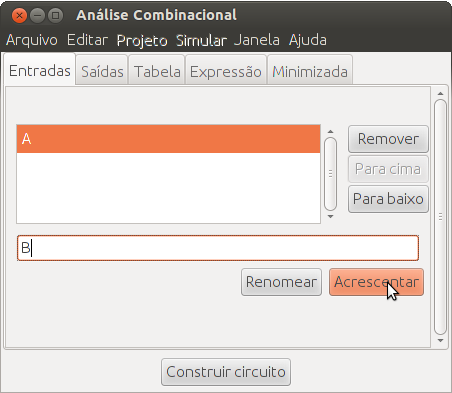
\includegraphics[height=7.4cm]{logisim.png}
\end{center}

Na aba ``Entradas'' adicione as variáveis de entrada. Em seguida, mude para
a aba saídas e adicione as variáveis de saída. A partir daí, você já pode
preencher a tabela na aba ``Tabela.'' Lembre-se que os estados que nunca
aparecem devem resultar em \emph{don't cares} nas saídas.
Após preencher a tabela, veja as expressões na aba ``Minimizada.''

\vfill

\noindent
$Y_2 =$ {\vcolor\hrulefill}

\vfill

\noindent
$Y_1 =$ {\vcolor\hrulefill}\\[16pt]
{\vcolor\hrulefill}

\vfill

\noindent
$Y_0 =$ {\vcolor\hrulefill}\\[16pt]
{\vcolor\hrulefill}

\end{multicols}

\newpage


Como uma alternativa, você pode usar mapas de Karnaugh para $5$ variáveis.\\[12pt]

\noindent
$Y_2 =$ {\vcolor\hrulefill}

\hfill
\scalebox{1}{
\begin{Karnaugh}{$B Q_2$}{\raisebox{0.5\baselineskip}{$Q_1 Q_0$}}
\node at (2,5.5) {$A = 0$};
\end{Karnaugh}
}
\hfill
\scalebox{1}{
\begin{Karnaugh}{$B Q_2$}{\raisebox{0.5\baselineskip}{$Q_1 Q_0$}}
\node at (2,5.5) {$A = 1$};
\end{Karnaugh}
}
\hspace*{\fill}

\noindent
$Y_1 =$ {\vcolor\hrulefill}

\hfill
\scalebox{1}{
\begin{Karnaugh}{$B Q_2$}{\raisebox{0.5\baselineskip}{$Q_1 Q_0$}}
\node at (2,5.5) {$A = 0$};
\end{Karnaugh}
}
\hfill
\scalebox{1}{
\begin{Karnaugh}{$B Q_2$}{\raisebox{0.5\baselineskip}{$Q_1 Q_0$}}
\node at (2,5.5) {$A = 1$};
\end{Karnaugh}
}
\hspace*{\fill}

\noindent
$Y_0 =$ {\vcolor\hrulefill}

\hfill
\scalebox{1}{
\begin{Karnaugh}{$B Q_2$}{\raisebox{0.5\baselineskip}{$Q_1 Q_0$}}
\node at (2,5.5) {$A = 0$};
\end{Karnaugh}
}
\hfill
\scalebox{1}{
\begin{Karnaugh}{$B Q_2$}{\raisebox{0.5\baselineskip}{$Q_1 Q_0$}}
\node at (2,5.5) {$A = 1$};
\end{Karnaugh}
}
\hspace*{\fill}

\noindent
\textbf{e)} Obtenha a expressão simplificada para a saída $P = ${\vcolor\rule{4cm}{0.4pt}}.

\vspace{-6pt}

\begin{center}
\scalebox{1.15}{
\begin{Karnaughvuit}{$Q_2$}{\raisebox{0.5\baselineskip}{$Q_1 Q_0$}}
  
\end{Karnaughvuit}
}
\end{center}

\vspace{-18pt}

\noindent
\textbf{f)} Construa o circuito da máquina de estados na próxima página.

\newpage

\noindent
\begin{tikzpicture}[x=0.4cm,y=0.4cm]
\draw[help lines,step=0.4cm,dashed,very thin,color={black!20!white}]
     (0,0) grid (42,64);
\end{tikzpicture}

\end{document}
